\documentclass[
	9pt, % Set the default font size, options include: 8pt, 9pt, 10pt, 11pt, 12pt, 14pt, 17pt, 20pt
	t, % Uncomment to vertically align all slide content to the top of the slide, rather than the default centered
	%aspectratio=169, % Uncomment to set the aspect ratio to a 16:9 ratio which matches the aspect ratio of 1080p and 4K screens and projectors
]{beamer}

\graphicspath{{Images/}{./}} % Specifies where to look for included images (trailing slash required)

\usepackage{booktabs} % Allows the use of \toprule, \midrule and \bottomrule for better rules in tables
\usepackage{graphicx}
\usepackage{caption}
\usepackage{subcaption}
\usepackage{hyperref}
\usepackage[english,brazil]{babel}
\usepackage{fontawesome5}
\usepackage{listings}
\usepackage{minted}
\usepackage{xcolor}
% \usepackage{graphicx}
% \usepackage{animate}
\RequirePackage[backend=biber,
style=ieee,
citestyle=authoryear,
]{biblatex}

% Define a custom command for an icon link
\newcommand{\iconLink}[2]{\href{#1}{\faLink \hspace{0.2em} {#2}}}
\newcommand{\yellowbox}[1]{\colorbox{yellow!75}{#1}}
\definecolor{darkgreen}{rgb}{0,0.5,0}

% Definindo um estilo para o destaque
%----------------------------------------------------------------------------------------
%	SELECT LAYOUT THEME
%----------------------------------------------------------------------------------------
\usetheme{Madrid}

%----------------------------------------------------------------------------------------
%	SELECT COLOR THEME
%----------------------------------------------------------------------------------------

% Beamer comes with a number of color themes that can be applied to any layout theme to change its colors. Uncomment each of these in turn to see how they change the colors of your selected layout theme.

%\usecolortheme{albatross}
%\usecolortheme{beaver}
%\usecolortheme{beetle}
% \usecolortheme{crane}
%\usecolortheme{dolphin}
%\usecolortheme{dove}
%\usecolortheme{fly}
%\usecolortheme{lily}
%\usecolortheme{monarca}
%\usecolortheme{seagull}
%\usecolortheme{seahorse}
%\usecolortheme{spruce}
%\usecolortheme{whale}
%\usecolortheme{wolverine}

%----------------------------------------------------------------------------------------
%	SELECT FONT THEME & FONTS
%----------------------------------------------------------------------------------------
\usefonttheme{default} % Typeset using the default sans serif font

%------------------------------------------------

\usepackage{palatino} % Use the Palatino font for serif text
\usepackage[default]{lato} % Use the Lato font for sans serif text

%----------------------------------------------------------------------------------------
%	SELECT INNER THEME
%----------------------------------------------------------------------------------------
\useinnertheme{rectangles}

%----------------------------------------------------------------------------------------
%	SELECT OUTER THEME
%----------------------------------------------------------------------------------------

% Outer themes change the overall layout of slides, such as: header and footer lines, sidebars and slide titles. Uncomment each theme in turn to see what changes it makes to your presentation.

%\useoutertheme{default}
%\useoutertheme{infolines}
%\useoutertheme{miniframes}
%\useoutertheme{smoothbars}
%\useoutertheme{sidebar}
%\useoutertheme{split}
%\useoutertheme{shadow}
%\useoutertheme{tree}
%\useoutertheme{smoothtree}

%\setbeamertemplate{footline} % Uncomment this line to remove the footer line in all slides
%\setbeamertemplate{footline}[page number] % Uncomment this line to replace the footer line in all slides with a simple slide count

%\setbeamertemplate{navigation symbols}{} % Uncomment this line to remove the navigation symbols from the bottom of all slides

% \bibliography{references} % Specifies the bibliography file to include publications
% \bibliographystyle{apalike} % Specifies the bibliography style
\addbibresource{references.bib}

%----------------------------------------------------------------------------------------
%	PRESENTATION INFORMATION
%----------------------------------------------------------------------------------------

\title[DesWebII]{Desenvolvimento Web II} % The short title in the optional parameter appears at the bottom of every slide, the full title in the main parameter is only on the title page
\subtitle{Aula 12 - \textit{Multi Tenancy}} % Presentation subtitle, remove this command if a subtitle isn't required
\author[Fabricio Bizotto]{Prof. Fabricio Bizotto} % Presenter name(s), the optional parameter can contain a shortened version to appear on the bottom of every slide, while the main parameter will appear on the title slide
\institute[IFC]{Instituto Federal Catarinense \\ \smallskip \textit{fabricio.bizotto@ifc.edu.br}} % Your institution, the optional parameter can be used for the institution shorthand and will appear on the bottom of every slide after author names, while the required parameter is used on the title slide and can include your email address or additional information on separate lines
\date[\today]{Ciência da Computação \\ \today} % Presentation date or conference/meeting name, the optional parameter can contain a shortened version to appear on the bottom of every slide, while the required parameter value is output to the title slide

%----------------------------------------------------------------------------------------
\begin{document}

%----------------------------------------------------------------------------------------
%	TITLE SLIDE
%----------------------------------------------------------------------------------------

\begin{frame}
	\titlepage % Output the title slide, automatically created using the text entered in the PRESENTATION INFORMATION block above
\end{frame}

%----------------------------------------------------------------------------------------
%	TABLE OF CONTENTS SLIDE
%----------------------------------------------------------------------------------------

\begin{frame}
	\frametitle{Roteiro} % Slide title, remove this command for no title
	
	\tableofcontents % Output the table of contents (all sections on one slide)
	%\tableofcontents[pausesections] % Output the table of contents (break sections up across separate slides)
\end{frame}

%----------------------------------------------------------------------------------------
%	PRESENTATION BODY SLIDES
%----------------------------------------------------------------------------------------

\section{Definição}

\begin{frame}
	\frametitle{Multi Tenancy}
	\framesubtitle{Definição}

	\begin{itemize}
		\item \textit{Multi Tenancy} é um padrão de arquitetura de software onde uma única instância de software serve a múltiplos clientes, chamados de \textit{tenants}.
		\item Cada \textit{tenant} é isolado dos demais, e pode ter suas próprias configurações, dados e personalizações.
		\item O \textit{Multi Tenancy} é comum em sistemas de \textit{Software as a Service} (SaaS), onde um único sistema é utilizado por múltiplos clientes.
		\item O \textit{Multi Tenancy} pode ser implementado em diferentes níveis de um sistema, como banco de dados, aplicação, interface de usuário, etc.
	\end{itemize}

	\begin{block}{Empresas que Utilizam \textit{Multi Tenancy}}
		\begin{itemize}
			\item \textbf{Salesforce:} um único sistema de CRM utilizado por milhares de empresas.
			\item \textbf{Google Apps:} um único sistema de e-mail, calendário, etc., utilizado por milhões de usuários.
			\item \textbf{Shopify:} um único sistema de e-commerce utilizado por milhares de lojas.
			\item \textbf{Microsoft 365:} um único sistema de produtividade utilizado por milhões de usuários.
			\item \textbf{Dropbox:} um único sistema de armazenamento de arquivos utilizado por milhões de usuários.
		\end{itemize}
	\end{block}

\end{frame}

\section{Analogia com Imóveis}

\begin{frame}
	\frametitle{Multi Tenancy}
	\framesubtitle{Analogia com Imóveis}
	
	\begin{columns}
		\column{0.5\textwidth}
		\begin{itemize}
			\item Imagine um prédio de apartamentos.
			\item Cada apartamento é um \textit{tenant}.
			\item Cada apartamento tem suas próprias chaves, móveis, decoração, etc.
			\item Cada apartamento é isolado dos demais.
			\item O prédio é o sistema de \textit{Multi Tenancy}.
		\end{itemize}

		\column{0.5\textwidth}
		\begin{figure}
			\centering
			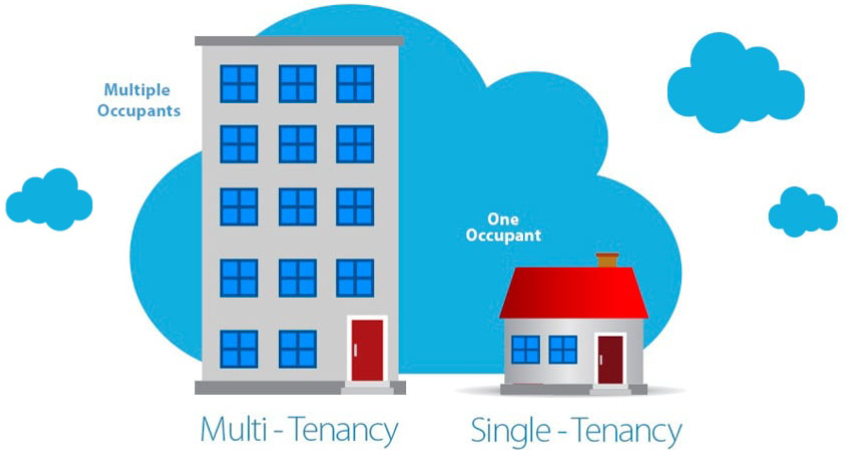
\includegraphics[width=0.9\textwidth]{multitenancy_imoveis.jpg}
			\caption{Single Tenant vs. Multi Tenant}
		\end{figure}

	\end{columns}

	\begin{block}{Não é a mesma coisa que \textit{Multi User}?}
		Não. Todos sistema \textit{Multi Tenant} é \textit{Multi User}, mas nem todo sistema \textit{Multi User} é \textit{Multi Tenant}.
	\end{block}

\end{frame}

\begin{frame}
	\frametitle{Multi Tenancy}
	\framesubtitle{Aplicação Multi User}

	\begin{columns}
		\column{0.5\textwidth}
		\begin{enumerate}
			\item Existe compartilhamento de dados e recursos entre os usuários.
			\item O professor pode ver e interagir com os dados dos alunos.
			\item O aluno pode ver suas próprias notas.
			\item O coordenador pode gerenciar as disciplinas, alunos, professores.
			\item Não existe isolamento entre os usuários.
			\item Não posso vender esse produto para outra escola.
		\end{enumerate}

		\column{0.5\textwidth}
		\begin{figure}
			\centering
			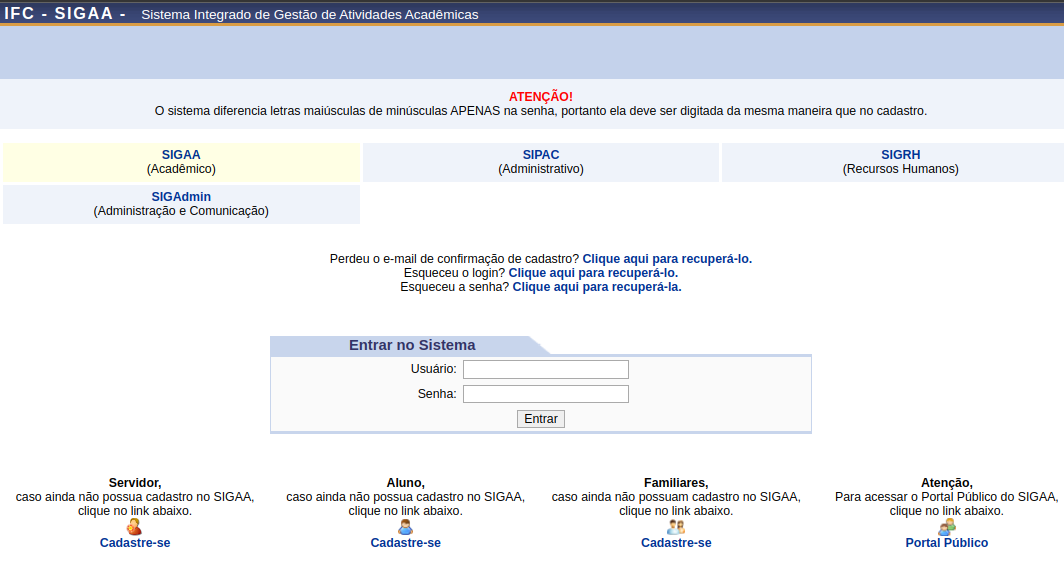
\includegraphics[width=0.9\textwidth]{sigaa_tela.png}
			\caption{Aplicação Multi User}
		\end{figure}

	\end{columns}

\end{frame}

\section{\textit{Single Tenant} vs. \textit{Multi Tenant}}

\begin{frame}
	\framesubtitle{\textit{Multi Tenant}}
	\frametitle{Single Tenant}

	\begin{block}{Definição}
		Aplicação que serve a um único cliente. Cada cliente tem sua própria instância da aplicação. Cada instância é isolada das demais.
	\end{block}

	\begin{exampleblock}{Vantagens}
		\begin{itemize}
			\item A base de dados é isolada. Maior segurança.
			\item A performance é previsível. Não será afetada por outros clientes.
			\item Facilidade para customizar a aplicação para um cliente específico.
			\item Oferece maior controle sobre a aplicação.
		\end{itemize}
	\end{exampleblock}

	\begin{alertblock}{Desvantagens}
		\begin{itemize}
			\item Cliente precisa arcar com os custos de uma instância completa.
			\item Exige maior esforço para manter e atualizar as instâncias.
		\end{itemize}
	\end{alertblock}

\end{frame}

\begin{frame}
	\frametitle{\textit{Single Tenant} vs. \textit{Multi Tenant}}
	\framesubtitle{\textit{Multi Tenant}}

	\begin{block}{Definição}
		Aplicação que serve a múltiplos clientes. Todos os clientes compartilham a mesma instância da aplicação. Cada cliente é isolado dos demais.
	\end{block}

	\begin{exampleblock}{Vantagens}
		\begin{itemize}
			\item Redução de custos. A aplicação é compartilhada entre os clientes.
			\item Facilidade para manter e atualizar a aplicação.
			\item Facilidade para escalar a aplicação.
			\item Facilidade para adicionar novos clientes.
		\end{itemize}
	\end{exampleblock}

	\begin{alertblock}{Desvantagens}
		\begin{itemize}
			\item Menor controle sobre a aplicação.
			\item Menor segurança. Um cliente pode afetar a performance de outros.
			\item Dificuldade para customizar a aplicação para um cliente específico.
		\end{itemize}
	\end{alertblock}

\end{frame}

\section{Tipos de \textit{Multi Tenancy}}

\begin{frame}
	\frametitle{Multi Tenancy}
	\framesubtitle{Tipos de \textit{Multi Tenancy}}

	Esses são os tipos mais comuns de \textit{Multi Tenancy}:

	\begin{itemize}
		\item \textbf{Shared Database:} todos os \textit{tenants} compartilham a mesma base de dados, tabelas, etc. Cada \textit{tenant} tem suas próprias linhas de dados. Essa é a forma mais básica de \textit{Multi Tenancy}.
		\item \textbf{One Schema Per Tenant:} todos os \textit{tenants} compartilham a mesma base de dados, mas cada \textit{tenant} tem seu próprio \textit{schema}. Cada \textit{tenant} tem suas próprias tabelas, índices, etc.
		\item \textbf{One Database Per Tenant:} cada \textit{tenant} tem sua própria base de dados. Cada \textit{tenant} tem suas próprias tabelas, índices, etc. É o mais seguro, mas também o mais caro.
	\end{itemize}

	% \begin{figure}
	% 	\centering
	% 	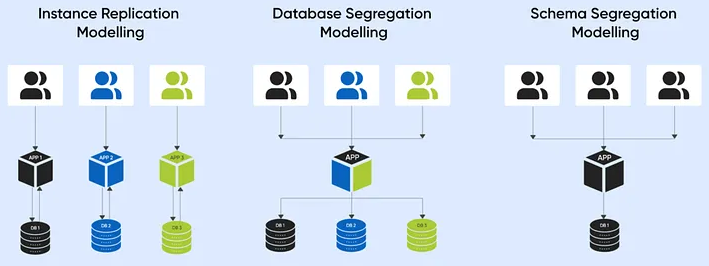
\includegraphics[width=0.8\textwidth]{tenancy_types.png}
	% 	% \caption{Tipos de \textit{Multi Tenancy}}
	% \end{figure}

\end{frame}

\subsection{Schema Database}

\begin{frame}
	\frametitle{Multi Tenancy}
	\framesubtitle{Schema Database}

	\begin{itemize}
		\item Somente um banco de dados é utilizado.
		\item Gerenciamento simples.
		\item É a forma mais comum de \textit{Multi Tenancy}.
		\item \alert{Aumenta os riscos de segurança ao expor dados de um \textit{tenant} para outro.}
		\item \alert{Não tem isolamento físico entre os \textit{tenants}.} Esse isolamento está na mão do desenvolvedor.
		
	\end{itemize}

	\begin{figure}
		\centering
		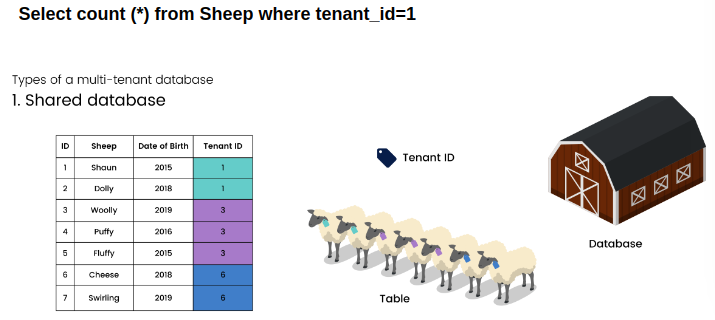
\includegraphics[width=0.9\textwidth]{schema_database.png}
		\caption{Schema Database}
	\end{figure}

\end{frame}

\subsection{One Schema Per Tenant}

\begin{frame}
	\frametitle{Multi Tenancy}
	\framesubtitle{One Schema Per Tenant}

	\begin{itemize}
		\item Cada \textit{tenant} tem seu próprio \textit{schema}.
		\item Os dados de cada \textit{tenant} estão isolados, mas compartilham a mesma base de dados.
		\item Reduz os riscos de segurança pois não precisa usar a cláusula \texttt{WHERE} para filtrar os dados entre os \textit{tenants}.
		\item \alert{Risco de consultar o \textit{schema} errado.}
	\end{itemize}

	\begin{figure}
		\centering
		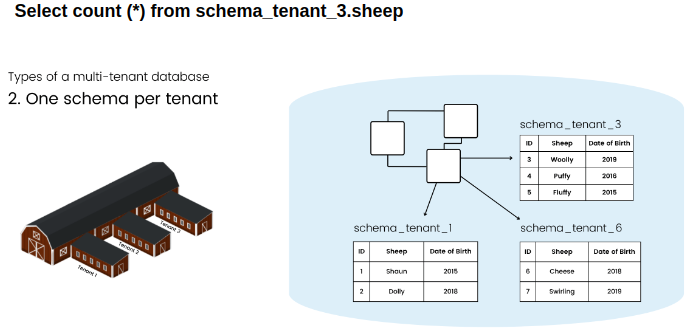
\includegraphics[width=0.9\textwidth]{one_schema.png}
		\caption{One Schema Per Tenant}
	\end{figure}

\end{frame}

\subsection{One Database Per Tenant}

\begin{frame}
	\frametitle{Multi Tenancy}
	\framesubtitle{One Database Per Tenant}

	\begin{itemize}
		\item Cada \textit{tenant} tem seu próprio banco de dados.
		\item Normalmente é usado para isolar um cliente grande.
		\item Maior segurança e isolamento entre os \textit{tenants}.
		\item Sem complexidade para filtrar os dados.
		\item \alert{Maior custo de manutenção e infraestrutura.}
		\item \alert{Alterações no banco de dados precisam ser replicadas para todos os \textit{tenants}.}
	\end{itemize}

	\begin{figure}
		\centering
		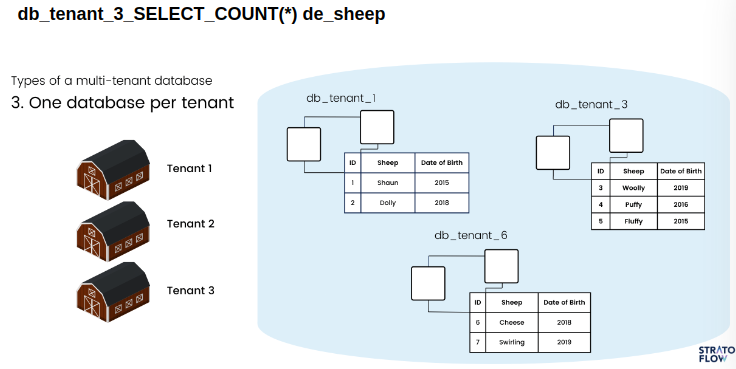
\includegraphics[width=0.8\textwidth]{one_per_database.png}
		\caption{One Database Per Tenant}
	\end{figure}

\end{frame}

\section{\textit{Multi Tenancy} em uma API REST}

\begin{frame}
	\frametitle{Multi Tenancy}
	\framesubtitle{\textit{Multi Tenancy} em uma API REST}

	\begin{itemize}
		\item Identificação do \textit{tenant} baseada em parâmetros de consulta\\
		\texttt{GET /api/v1/tasks?tenant=tenant\_id}
		\item Identificação do \textit{tenant} baseada em subdomínio\\
		\texttt{GET https://tenant1.myapp.com/api/v1/tasks}
		\item Identificação do \textit{tenant} baseada na URL\\
		\texttt{GET https://myapp.com/tenant1/api/v1/tasks}
	\end{itemize}

\end{frame}

\section{Considerações Finais}

\begin{frame}
	\frametitle{Multi Tenancy}
	\framesubtitle{Considerações Finais}

	\begin{itemize}
		\item O \textit{Multi Tenancy} é uma forma de compartilhar recursos entre múltiplos clientes.
		\item Existem diferentes formas de implementar o \textit{Multi Tenancy}, cada uma com suas vantagens e desvantagens.
		\item O \textit{Multi Tenancy} é comum em sistemas de \textit{Software as a Service} (SaaS).
		\item O \textit{Multi Tenancy} é uma forma de reduzir custos e facilitar a manutenção e atualização de sistemas.
		\item O \textit{Multi Tenancy} é uma forma de escalar sistemas para atender a um grande número de clientes.
	\end{itemize}

\end{frame}

\section{QUIZ}

\begin{frame}
	\frametitle{Recapitulando}
	\framesubtitle{QUIZ}

	Vamos praticar um pouco o que vimos até agora?
	\vfill

	\bigskip
	\centering

	\href{https://quizizz.com/admin/quiz/65c20cca036b2c1121fc8392?source=admin&trigger=quizPage}{\textbf{QUIZ - Multi Tenancy}}
	\vfill
		
\end{frame}

%----------------------------------------------------------------------------------------

\section{Experimentos}

\begin{frame}
	\frametitle{Experimentos}
	\framesubtitle{Vamos praticar?}

	Nesta atividade, o aluno deve desenvolver uma aplicação web simples utilizando a arquitetura multi tenancy. O objetivo é criar uma plataforma de lista de tarefas compartilhada, onde diferentes usuários, ou inquilinos, podem criar e gerenciar suas próprias listas de tarefas dentro da mesma instância da aplicação, garantindo o isolamento e a segurança dos dados de cada inquilino. Os participantes devem planejar e projetar a aplicação, implementar a lógica da aplicação com recursos como autenticação de usuário, gerenciamento de tarefas e compartilhamento de listas.
	
	\bigskip
	
	A entrega no incluirá o código-fonte da aplicação (GitHub) e documentação de suporte (README.md).

\end{frame}

\end{document} 
